\documentclass{article}

% NeurIPS 2026 Evaluations & Datasets Track (single-blind)
\usepackage[eandd, nonanonymous]{neurips_2026}

\usepackage[utf8]{inputenc}
\usepackage[T1]{fontenc}
\usepackage{hyperref}
\usepackage{url}
\usepackage{booktabs}
\usepackage{amsfonts}
\usepackage{amsmath}
\usepackage{amssymb}
\usepackage{amsthm}
\usepackage{nicefrac}
\usepackage{xcolor}
\usepackage{enumitem}
\usepackage{mathtools}
\usepackage{graphicx}
\usepackage{tikz}
\usetikzlibrary{positioning, arrows.meta}

\newtheorem{theorem}{Theorem}[section]
\newtheorem{proposition}[theorem]{Proposition}
\newtheorem{corollary}[theorem]{Corollary}
\theoremstyle{definition}
\newtheorem{definition}[theorem]{Definition}
\newtheorem{example}[theorem]{Example}
\newtheorem{remark}[theorem]{Remark}

\newcommand{\D}{\mathcal{D}}
\newcommand{\Dm}{\mathcal{D}^{-}}
\newcommand{\Dfull}{\mathcal{D}^{\mathrm{full}}}
\newcommand{\HB}{\mathcal{H}_B}
\newcommand{\HU}{\mathcal{H}_U}
\newcommand{\Hcand}{\mathcal{H}_{\mathrm{cand}}}
\newcommand{\Hgold}{\mathcal{H}^{*}}
\newcommand{\Rgold}{\mathcal{H}^{*}_3}
\newcommand{\La}{\mathcal{L}}
\newcommand{\Rs}{R_s}
\newcommand{\Rd}{R_d}
\newcommand{\Rdf}{R_{df}}
\newcommand{\Rdexc}{R_d^{\mathrm{exc}}}
\newcommand{\Rdfspace}{\mathcal{R}_{df}}
\newcommand{\Rdexcspace}{\mathcal{R}_{d}^{\mathrm{exc}}}
\newcommand{\partfunc}{\kappa}
\newcommand{\pred}{\mathrm{pred}}
\newcommand{\head}{\mathrm{head}}
\newcommand{\Supp}{\mathrm{Supp}}
\newcommand{\Crit}{\mathrm{Crit}}
\newcommand{\CritStar}{\mathrm{Crit}^{*}}
\newcommand{\Exp}{\mathrm{Exp}}
\newcommand{\Nov}{\mathrm{Nov}}
\newcommand{\proves}{\vdash}
\newcommand{\pDelta}{\vdash_{\Delta}}
\newcommand{\pPartial}{\vdash_{\partial}}
\newcommand{\pSLD}{\vdash_{\mathrm{SLD}}}
\newcommand{\defto}{\Rightarrow}
\newcommand{\strictto}{\rightarrow}
\newcommand{\defeatto}{\leadsto}
\newcommand{\comp}[1]{\overline{#1}}


\title{DeFAb: A Defeasible Abduction Benchmark for Evaluating\\Grounding, Novelty, and Belief Revision in Foundation Models}

\author{%
  Patrick Cooper \\
  Department of Computer Science\\
  University of Colorado Boulder\\
  Boulder, CO 80309 \\
  \texttt{patrick.cooper@colorado.edu} \\
}


\begin{document}

\maketitle


\begin{abstract}
Foundation models excel at forward inference but struggle with abduction and belief revision: proposing hypotheses that explain observations and retracting defaults when exceptions arise. We introduce \textsc{DeFAb} (Defeasible Abduction Benchmark), a dataset and generation pipeline that converts legacy knowledge bases into defeasible theories and generates evaluation instances with polynomial-time verifiable gold-standard hypotheses. The pipeline pairs taxonomic hierarchies from publicly funded knowledge bases (OpenCyc, YAGO, Wikidata) with behavioral property graphs (ConceptNet, UMLS) to produce defeasible rules and defeaters at scale. Instances are stratified into three levels: fact completion, rule abduction, and defeater abduction, where models must construct conservative exception rules that override incorrect defaults while preserving unrelated expectations. The dataset comprises 372,402 instances across 33.7 million materialized rules from 15 knowledge sources spanning biology, law, materials science, chemistry, commonsense reasoning, and biomedical informatics (including 29.5 million rules from UMLS). A synthetic contamination control generates structurally isomorphic theories with invented predicate names, isolating formal reasoning from memorized associations. Evaluation of four frontier models reveals that grounding is largely solved at Level~2 (73--79\% accuracy) while belief revision at Level~3 remains highly prompt-sensitive, with a 56--79 percentage-point swing between direct and chain-of-thought prompting for reasoning-optimized models. The dataset, generation pipeline, and evaluation harness are released under the MIT license.
\end{abstract}


%% ====================================================================
\section{Introduction}\label{sec:intro}
%% ====================================================================

The challenge of creative AI extends beyond distributional sparsity. Transformational discoveries do not simply extend existing knowledge; they often contradict it. A striking example from biology is intrinsically disordered proteins (IDPs): proteins that lack fixed three-dimensional structure yet remain functionally essential~\cite{dunker2001intrinsically}. Prior to this discovery, the prevailing dogma held that proteins required stable 3D conformations to perform biological functions. An AI trained on data reflecting this conventional wisdom would be unlikely to hypothesize the existence of IDPs, because the hypothesis directly contradicts the domain knowledge encoded in its training corpus.

This failure reflects three entangled deficits in current foundation models. The first is a \textit{grounding deficit}: models lack an explicit epistemic structure distinguishing strict knowledge from revisable defaults, and cannot trace predictions to their supporting evidence. The second is a \textit{novelty deficit}: without knowing which beliefs are revisable, models cannot identify where creative exceptions might apply. The third is a \textit{belief revision deficit}: even when models update their knowledge, they lack the formal machinery to ensure the principle of minimal change~\cite{alchourron1985logic}: accommodating new evidence while disturbing as few existing commitments as possible. The IDP discovery illustrates all three: the creative act requires not merely asserting that disordered proteins exist, but doing so via a targeted revision that overrides the structure--function default for a specific subclass while leaving predictions about conventionally structured proteins intact.

\textit{Defeasible reasoning} provides exactly this structure. In a defeasible theory, every conclusion is derived through a traceable chain of strict and defeasible rules, every default is explicitly revisable, and every piece of evidence participates in identifiable support sets. This provides grounding, the machinery for novelty, and a concrete operationalization of rational belief revision: our conservativity requirement (Definition~\ref{def:conserv}) ensures that resolutions preserve all expectations except the targeted anomaly, directly implementing AGM's minimal change postulate~\cite{gardenfors1988knowledge, katsuno1991propositional}.

Current benchmarks leave this space largely untested. Entailment verification tasks~\cite{tafjord2021proofwriter} evaluate forward, monotonic reasoning. Knowledge editing benchmarks such as CounterFact~\cite{meng2022locating} measure whether a target fact changed but rely on ad hoc heuristics for side-effect assessment rather than formally verifying conservativity. What is missing is a principled method for generating grounded abductive instances: one that combines the expressivity of defeasible logic with verifiable gold-standard answers and formal revision guarantees.

A further challenge is the \textit{contamination confound}. For well-documented defaults and exceptions appearing in textbooks (``birds fly'' / ``penguins do not fly''), we cannot distinguish genuine defeasible reasoning from retrieval of memorized training-corpus solutions. GSM1K~\cite{zhang2024gsm1k} demonstrated accuracy drops attributable to contamination, and LiveCodeBench~\cite{jain2025livecodebench} revealed contamination even in frontier models via time-segmented evaluation. For defeasible reasoning benchmarks grounded in well-known knowledge bases, the risk is acute.

We introduce \textsc{DeFAb} (\textbf{De}feasible \textbf{A}bduction \textbf{B}enchmark), a dataset and generation pipeline grounded in this approach. Our contributions are:

\begin{enumerate}[label=(\arabic*),nosep]
    \item \textbf{A dataset and generation pipeline} for converting definite logic programs into defeasible theories via a parameterized partition function $\partfunc$ that controls which clauses are strict versus revisable, with polynomial-time instance generation producing evaluation tasks at three difficulty levels: fact completion, rule abduction, and defeater abduction with formal conservativity guarantees.

    \item \textbf{A cross-ontology knowledge base extraction methodology} for generating defeasible rule bases at scale from heterogeneous publicly funded knowledge sources. The procedure pairs taxonomic hierarchies with behavioral property graphs to synthesize defeasible rules; exception relations serve as structured defeater sources, enabling automatic instance generation without manual authoring. The dataset spans 15 knowledge sources and 33.7 million materialized rules.

    \item \textbf{A synthetic contamination control.} Procedurally generated theories with invented predicate names preserve structural parameters of naturalistic theories while guaranteeing that gold-standard hypotheses fall outside any pretraining corpus. The naturalistic--synthetic accuracy gap provides a per-model upper bound on contamination-attributable performance inflation.

    \item \textbf{Baseline evaluation of four frontier models} revealing a rich capability structure: grounding is largely solved (73--79\% at Level~2) while belief revision is latent and prompt-sensitive, with an architectural dissociation between reasoning-optimized and instruction-optimized models.

    \item \textbf{A multimodal visual grounding modality (M5)} that extends the rendering protocol to vision-language evaluation, replacing or supplementing textual entity identification with images harvested from linked knowledge bases (Wikidata P18, VisualSem, BabelNet). This provides the first defeasible reasoning benchmark with formally verified gold standards for vision-language models, connecting to recent findings that VLMs systematically fail on atypical instances~\cite{park2025visage}---precisely the entities governed by defeater rules.
\end{enumerate}


%% ====================================================================
\section{Related Work}\label{sec:related}
%% ====================================================================

\paragraph{Non-monotonic reasoning.}
Reiter's default logic~\cite{reiter1980logic} and McCarthy's circumscription~\cite{mccarthy1980circumscription} addressed the inadequacy of classical logic for commonsense reasoning. Nute's defeasible logic~\cite{nute1987defeasible, nute1994defeasible} offered a computationally tractable alternative, and the KLM framework~\cite{kraus1990nonmonotonic} provided axiomatic foundations for rational non-monotonic inference. The proof theory we adopt follows Antoniou et al.~\cite{antoniou2001defeasible}, who established that propositional defeasible derivation has linear time complexity~\cite{maher2001propositional}, a result that underlies the tractability of our generation pipeline.

\paragraph{Belief revision.}
Our framework connects to the theory initiated by Alchourr\'{o}n, G\"{a}rdenfors, and Makinson~\cite{alchourron1985logic}, who established rationality postulates for belief updating. Dalal~\cite{dalal1988investigations} introduced distance-based revision using Hamming distance between models. Our conservativity requirement operationalizes minimal change in the defeasible setting, and our revision distance provides a tractable analogue of Dalal's distance. The knowledge editing literature (ROME~\cite{meng2022locating}, MEMIT~\cite{meng2023mass}, and evaluations of their side effects~\cite{cohen2024evaluating}) addresses belief revision in neural models but lacks formally grounded measures of conservativity.

\paragraph{Existing benchmarks.}
ProofWriter~\cite{tafjord2021proofwriter} and LogicNLI~\cite{tian2021diagnosing} evaluate deductive verification. The INABHYD benchmark~\cite{inabhyd2025} demonstrates that language models fail to follow Occam's Razor in abductive contexts. LogiDynamics~\cite{zheng2025logidynamics} studies the interplay of inductive, abductive, and deductive inference but evaluates over generic analogical tasks rather than formally specified defeasible theories. The closest related work is \textsc{DeFReasing}~\cite{allaway2025defreasing}, which probes whether language models correctly handle property inheritance with exceptions. Our benchmark differs in three fundamental ways: \textsc{DeFAb} is a \emph{construction} task (the model must generate the exception rule), uses formally specified theories with verifier-backed gold standards, and includes a conservativity check operationalizing AGM minimal change.

\paragraph{Knowledge base provenance.}
The 1980s produced large-scale knowledge bases from government AI programs: Japan's FGCS project~\cite{fuchi1984aiming, feigenbaum1993fgcs}, the UK's Alvey Programme~\cite{alvey1985ikbs}, and Cyc~\cite{lenat1990cyc, lenat1995cyc}. This tradition continued through NSF-funded resources (WordNet~\cite{miller1995wordnet}, ConceptNet~\cite{speer2017conceptnet}), NIH programs (UMLS~\cite{lindberg1993umls}, Gene Ontology~\cite{ashburner2000go}), EU-funded ontologies (LKIF Core~\cite{lkif2007}, BabelNet~\cite{navigli2012babelnet}), and encyclopedic projects (Wikidata~\cite{vrandecic2014wikidata}, DBpedia~\cite{lehmann2015dbpedia}, YAGO~\cite{suchanek2024yago}). These systems encode both default generalizations and documented exceptions, making them natural sources for defeasible rules and structured defeaters.

\paragraph{Contamination-aware evaluation.}
Zhang et al.~\cite{zhang2024gsm1k} demonstrated contamination effects in grade-school math, and LiveCodeBench~\cite{jain2025livecodebench} revealed contamination in code evaluation through time-segmented problems. Our synthetic contamination control provides the first contamination-resistant evaluation methodology for defeasible reasoning.


%% ====================================================================
\section{DeFAb: Dataset Design}\label{sec:design}
%% ====================================================================

\begin{figure}[t]
\centering
\resizebox{\textwidth}{!}{% DeFAb combined pipeline + L1/L2/L3 generation figure
%
% Fixed-grid layout with conservative row heights:
%   Every row uses anchor=north with an ABSOLUTE y coordinate.
%   minimum height is set ≥ actual content height so boxes never overflow.
%
%   Row y-coordinates (top of box):
%     Pipeline arc :  y = 0.00
%     Level headers :  y = −1.05   (height 0.40cm → bottom −1.45)
%     Theory boxes  :  y = −1.60   (height 0.90cm → bottom −2.50)  3 lines max
%     Ablated boxes :  y = −2.65   (height 0.70cm → bottom −3.35)  2 lines max
%     Gold boxes    :  y = −3.50   (height 0.45cm → bottom −3.95)  1 line
%     Distractor    :  y = −4.10   (height 0.40cm → bottom −4.50)  1 line
%     Modality      :  y = −4.65   (height 0.60cm → bottom −5.25)  M5 taller
%     Caption label :  y = −5.40
%
%   Column x-centres: L1=−3.50, L2=0, L3=+3.50
%
\begin{tikzpicture}[
    >=stealth,
    %--- pipeline top row ---
    pipebox/.style={
        draw=defabBlue!70, rounded corners=2pt,
        font=\fontsize{6.2}{7.2}\selectfont,
        inner sep=3pt, text centered, align=center,
        fill=defabBlue!6, line width=0.4pt,
        minimum height=0.54cm, text width=1.30cm
    },
    %--- column headers ---
    levhdr/.style={
        draw=defabTeal!70, rounded corners=2pt,
        font=\fontsize{6.5}{7.5}\selectfont\bfseries,
        inner sep=2.5pt, text centered, align=center,
        fill=defabTeal!12, line width=0.4pt,
        text width=3.2cm, minimum height=0.40cm,
        anchor=north, text=defabTeal
    },
    %--- theory box (3 lines strict) ---
    tbox/.style={
        draw=defabGray!45, rounded corners=1.5pt,
        font=\fontsize{5.6}{6.6}\selectfont,
        inner sep=2.5pt, align=left,
        fill=white, line width=0.35pt,
        text width=3.2cm, minimum height=0.90cm, anchor=north
    },
    %--- ablated element box (2 lines, red) ---
    abox/.style={
        draw=defabRed!65, rounded corners=1.5pt,
        font=\fontsize{5.6}{6.6}\selectfont\bfseries,
        inner sep=2.5pt, align=left,
        fill=defabRed!7, line width=0.45pt,
        text width=3.2cm, minimum height=0.70cm,
        anchor=north, text=defabRed
    },
    %--- gold answer box (1 line, teal) ---
    gbox/.style={
        draw=defabTeal!70, rounded corners=1.5pt,
        font=\fontsize{5.6}{6.6}\selectfont\bfseries,
        inner sep=2.5pt, align=left,
        fill=defabTeal!9, line width=0.40pt,
        text width=3.2cm, minimum height=0.45cm,
        anchor=north, text=defabTeal!85
    },
    %--- distractor box (1 line, gray italic) ---
    dbox/.style={
        draw=defabGray!35, rounded corners=1.5pt,
        font=\fontsize{5.4}{6.2}\selectfont\itshape,
        inner sep=2.5pt, align=left,
        fill=defabGray!4, line width=0.30pt,
        text width=3.2cm, minimum height=0.40cm,
        anchor=north, text=defabGray
    },
    %--- modality boxes (gold border) ---
    mbox/.style={
        draw=defabGold!70, rounded corners=2pt,
        font=\fontsize{6.0}{7.0}\selectfont,
        inner sep=2.5pt, text centered, align=center,
        fill=defabGold!8, line width=0.4pt,
        text width=3.0cm, anchor=north
    },
    %--- image placeholder (for M5 example) ---
    imgbox/.style={
        draw=defabGold!60, rounded corners=1pt,
        font=\fontsize{5.0}{5.8}\selectfont\bfseries,
        inner sep=1.5pt, text centered, align=center,
        fill=defabGold!12, line width=0.5pt,
        minimum width=0.7cm, minimum height=0.42cm,
        text=defabGold!80
    },
    %--- arrows ---
    parr/.style={->, thick, color=defabBlue!55, line width=0.6pt},
    sarr/.style={->, thin, color=defabGray!60, line width=0.40pt},
]

%% ============================================================
%% PIPELINE ARC  (top row, centred)
%% ============================================================
\node[pipebox] (kb) at (-5.10, 0)
    {KBs\\{\fontsize{5}{6}\selectfont\color{defabGray}15+ srcs}};
\node[pipebox, right=0.45cm of kb] (lp) {Logic\\Program $\Pi$};
\node[pipebox, right=0.45cm of lp] (dt) {Defeasible\\Theory $\D$};
\node[pipebox, right=0.45cm of dt] (ab) {Ablate\\$e$};
\node[pipebox, right=0.45cm of ab] (vr) {\textbf{Verifier}\\$O(|\D|^3)$};

\draw[parr] (kb) -- node[above,font=\fontsize{4.8}{5.8}\selectfont\itshape,
    text=defabGray,inner sep=1pt]{form.} (lp);
\draw[parr] (lp) -- node[above,font=\fontsize{4.8}{5.8}\selectfont\itshape,
    text=defabGray,inner sep=1pt]{$\kappa$} (dt);
\draw[parr] (dt) -- node[above,font=\fontsize{4.8}{5.8}\selectfont\itshape,
    text=defabGray,inner sep=1pt]{ablate} (ab);
\draw[parr] (ab) -- node[above,font=\fontsize{4.8}{5.8}\selectfont\itshape,
    text=defabGray,inner sep=1pt]{verify} (vr);

%% ============================================================
%% LEVEL HEADERS  (top at y = −1.05)
%% ============================================================
\node[levhdr] at (-3.50,-1.05) (h1) {L1: Fact Completion};
\node[levhdr] at (  0.00,-1.05) (h2) {L2: Rule Abduction};
\node[levhdr] at (  3.50,-1.05) (h3) {L3: Defeater Abduction};

%% ============================================================
%% ROW 1 — Theory boxes  (top at y = −1.60, min-height 0.90cm)
%% All columns have exactly 3 content lines
%% ============================================================
\node[tbox] at (-3.50,-1.60) {
  \textbf{Theory:} \texttt{bear(G)\ bear(P)\ arc(P)}\\
  $r_d$: \texttt{bear(X)$\Rightarrow$hib(X)}\\
  $r^*$: \texttt{bear(X),arc(X)$\leadsto\neg$hib}
};
\node[tbox] at ( 0.00,-1.60) {
  \textbf{Theory:} \texttt{bear(G)\ bear(P)\ arc(P)}\\
  $r_s$: \texttt{bear(X)$\to$mammal(X)}\\
  $r^*$: \texttt{bear(X),arc(X)$\leadsto\neg$hib}
};
\node[tbox] at ( 3.50,-1.60) {
  \textbf{Theory:} \texttt{bear(P)\ arc(P)\ seal(P)}\\
  \texttt{winter\_active(P)}\\
  $r_d$: \texttt{bear(X)$\Rightarrow$hib(X)}
};

%% ============================================================
%% ROW 2 — Ablated boxes  (top at y = −2.65, min-height 0.70cm)
%% 2 content lines per box
%% ============================================================
\node[abox] at (-3.50,-2.65) {
  \textbf{Remove:} \texttt{bear(grizzly)}\\
  Target \texttt{hib(G)}: chain broken!
};
\node[abox] at ( 0.00,-2.65) {
  \textbf{Remove:} $r_d$: \texttt{bear(X)$\Rightarrow$hib}\\
  Target \texttt{hib(G)}: no rule!
};
\node[abox] at ( 3.50,-2.65) {
  \textbf{Remove:} $r^*$ — now $r_d$ fires\\
  $\Rightarrow$\texttt{hib(polar)}: \textbf{anomaly!}
};

%% ============================================================
%% ROW 3 — Gold answer boxes  (top at y = −3.50, min-height 0.45cm)
%% ============================================================
\node[gbox] at (-3.50,-3.50) {
  \textbf{Gold:} \texttt{bear(grizzly)} (restores)
};
\node[gbox] at ( 0.00,-3.50) {
  \textbf{Gold:} \texttt{bear(X)$\Rightarrow$hib(X)}
};
\node[gbox] at ( 3.50,-3.50) {
  \textbf{Score 1.0:} $r^*$ restored; $r^*\!\succ\!r_d$
};

%% ============================================================
%% ROW 4 — Distractor boxes  (top at y = −4.10, min-height 0.40cm)
%% ============================================================
\node[dbox] at (-3.50,-4.10) (d1) {
  Distractor: \texttt{mammal(G)} [wrong pred.]
};
\node[dbox] at ( 0.00,-4.10) (d2) {
  Distractor: \texttt{mammal(X)$\Rightarrow$hib} [too broad]
};
\node[dbox] at ( 3.50,-4.10) (d3) {
  Score 0.5: \texttt{$\neg$hib(X):- bear(X)} [not conserv.]
};

%% ============================================================
%% ROW 5 — Modality boxes  (top at y = −4.65, height varies)
%% M5 box is taller to show visual-grounding schematic
%% ============================================================
\node[mbox, minimum height=0.42cm] at (-3.50,-4.65) (m1) {M1 Narrative};
\node[mbox, minimum height=0.42cm] at ( 0.00,-4.65) (m2) {M2--M4 Formal};

%% M5 box with embedded image-placeholder schematic
\node[mbox, minimum height=0.72cm, text width=3.0cm] at (3.50,-4.65) (m3) {
  M5: Visual Grounding\\[-1pt]
  \texttt{bear(P).}\ $\to$\
  \begin{tikzpicture}[baseline=-1pt]
    \draw[defabGold!60, rounded corners=0.8pt, line width=0.45pt,
          fill=defabGold!12]
        (0,0) rectangle (0.72cm,0.36cm);
    \node[font=\fontsize{4.6}{5}\selectfont\bfseries,
          text=defabGold!80] at (0.36cm,0.18cm) {IMG};
    % small camera corner marks
    \draw[defabGold!50, line width=0.3pt] (0.05cm,0.30cm)
        -- (0.05cm,0.31cm) -- (0.12cm,0.31cm);
    \draw[defabGold!50, line width=0.3pt] (0.67cm,0.31cm)
        -- (0.67cm,0.30cm);
  \end{tikzpicture}
};

\draw[sarr] (d1.south) -- (m1.north);
\draw[sarr] (d2.south) -- (m2.north);
\draw[sarr] (d3.south) -- (m3.north);

%% horizontal sibling arrows between modality boxes
\draw[{<[scale=0.55]}-{>[scale=0.55]}, color=defabGold!65, line width=0.4pt]
    (m1.east) -- (m2.west);
\draw[{<[scale=0.55]}-{>[scale=0.55]}, color=defabGold!65, line width=0.4pt]
    (m2.east) -- (m3.west);

\node[font=\fontsize{5.0}{6}\selectfont\itshape, text=defabGold!80,
      anchor=north] at (0,-5.42)
    {Any instance rendered in five modalities (M5 replaces entity names with images)};

%% ============================================================
%% Arrows: pipeline ablation box → column headers
%% ============================================================
\draw[sarr] (ab.south) ..controls +(-0.30,-0.28) and +(0.12,0.30).. (h1.north);
\draw[sarr] (ab.south) -- (h2.north);
\draw[sarr] (ab.south) ..controls +(0.30,-0.28) and +(-0.12,0.30).. (h3.north);

\end{tikzpicture}
}
\caption{The DeFAb generation pipeline. Legacy knowledge bases are formalized as definite logic programs (Stage~1), converted to defeasible theories via partition function $\kappa$ (Stage~2), ablated to produce evaluation instances at three difficulty levels with polynomial-time gold-standard verification (Stage~3), and rendered into five modalities for evaluation (Stage~4). Full formal definitions appear in Appendix~\ref{app:definitions}.}
\label{fig:pipeline}
\end{figure}


%% --------------------------------------------------------------------
\subsection{Source Theories}\label{subsec:source}
%% --------------------------------------------------------------------

We formalize legacy knowledge bases as definite logic programs over a first-order signature $\Sigma = (\mathcal{C}, \mathcal{F}, \mathcal{P})$. A definite logic program $\Pi$ is a finite set of clauses $h \leftarrow b_1, \ldots, b_n$ ($n \geq 0$). Its semantics is given by the least Herbrand model $\mathcal{M}_\Pi = \mathrm{lfp}(T_\Pi)$. The key property is monotonicity: $\Pi \subseteq \Pi'$ implies $\mathcal{M}_\Pi \subseteq \mathcal{M}_{\Pi'}$. This is precisely the limitation our framework addresses: monotonic theories cannot retract defaults in light of new evidence.


%% --------------------------------------------------------------------
\subsection{Defeasible Conversion}\label{subsec:conversion}
%% --------------------------------------------------------------------

A defeasible theory $\D = (F, \Rs, \Rd, \Rdf, {\succ})$ consists of facts~$F$, strict rules~$\Rs$, defeasible rules~$\Rd$, defeaters~$\Rdf$, and an acyclic superiority relation~$\succ$ (Definition~\ref{def:deftheory}). A literal $q$ is defeasibly provable, written $\D \pPartial q$, when there exists an applicable defeasible rule for $q$ and every attacking rule for $\comp{q}$ is either inapplicable or overridden by a superior rule (Definition~\ref{def:defderiv}).

We convert a definite logic program $\Pi$ into a defeasible theory via a partition function $\partfunc: \Pi \to \{s, d\}$:
\begin{equation}\label{eq:conversion}
    \phi_\partfunc(\Pi) = (F_\partfunc,\; \Rs^{\partfunc},\; \Rd^{\partfunc},\; \emptyset,\; \emptyset).
\end{equation}
Clauses assigned~$s$ become facts or strict rules; clauses assigned~$d$ become defeasible rules. The converted theory has empty defeater and superiority components: generating these is the task we pose to the model.

We study five structured partition families: the leaf partition ($\partfunc_{\mathrm{leaf}}$, facts defeasible), the rule partition ($\partfunc_{\mathrm{rule}}$, rules defeasible), the depth-$k$ partition ($\partfunc_{\mathrm{depth}}(k)$), a random baseline ($\partfunc_{\mathrm{rand}}(\delta)$), and the \emph{type-grounded partition} $\partfunc_{\mathrm{type}}$ which maps relation type to epistemic status: taxonomic edges are strict, capability assertions are defeasible, and exception relations seed $\Rdf$ directly. When all clauses are strict, the conversion is conservative: $q \in \mathcal{M}_\Pi \iff \D_\partfunc \pDelta q$ (Proposition~\ref{prop:strict}).


%% --------------------------------------------------------------------
\subsection{Three-Level Instance Generation}\label{subsec:instances}
%% --------------------------------------------------------------------

Given a converted theory $\D$ and a derivable target $q$, we generate evaluation instances by exploiting the grounding structure. An element $e$ is full-theory critical if $\D \setminus \{e\} \not\pPartial q$; this is decidable in polynomial time. We ablate a critical element to form $\Dm = \D \setminus \{e\}$, inject $k = 5$ syntactically similar distractors, and define the gold set $\Hgold = \{h \mid \Dm \cup \{h\} \pPartial q,\; h \text{ minimal}\}$. Instances are stratified:

\textit{Level 1 (Fact completion).} The ablated element is a ground fact ($e \in F$). The model must identify the missing observation.

\textit{Level 2 (Rule abduction).} The ablated element is a defeasible rule ($e \in \Rd$). The model must reconstruct a missing generalization from candidates including syntactically similar distractors.

\textit{Level 3 (Defeater abduction).} The theory actively derives a prediction $\comp{\alpha}$ via defeasible rules, but the observation $\alpha$ contradicts it. The model must construct a novel defeater or exception rule that resolves the anomaly while preserving unrelated expectations. A resolution is \textit{conservative} if it preserves all expectations except $\comp{\alpha}$ (Definition~\ref{def:conserv}): our operationalization of AGM minimal change.

We measure resolutions via predicate novelty $\Nov(r, \Dm)$, revision distance $d_{\mathrm{rev}}$, and a five-level graded scoring function that decomposes failures along the stages of rational belief revision (Section~\ref{subsec:scoring}).

\paragraph{Gold-standard generation for Level~3.}
We work backwards from a complete theory $\Dfull$ that already contains the resolution $r^*$, remove $r^*$ and its superiority assertions to form a challenge theory $\Dm$, verify that $\alpha$ becomes anomalous, and compute the gold set of all conservative resolutions. Gold hypotheses are obtained through three mechanisms: (i)~automated extraction from ConceptNet \texttt{NotCapableOf} assertions and Wikidata P2303 constraint--exception pairs; (ii)~expert cross-validation against LKIF Core, MatOnto, and YAGO constraints; (iii)~domain-expert authoring for high-novelty instances.


%% --------------------------------------------------------------------
\subsection{Rendering and Evaluation Protocol}\label{subsec:rendering}
%% --------------------------------------------------------------------

A rendering codec $\rho = (\rho_{\mathrm{enc}}, \rho_{\mathrm{dec}})$ translates between formal theories and natural language. We define five encoding modalities: narrative (M1), semi-formal (M2), annotated formal (M3), pure formal (M4), and visual grounding (M5, Section~\ref{subsec:m5}). M1--M4 are text-only modalities trading naturalness against faithfulness; M5 introduces a cross-modal dimension that grounds entity identification in images while retaining M4 formal syntax for theory rules, target, and candidates. The decoder maps model outputs back to formal rules via exact match (D1), template extraction (D2), or semantic parsing (D3), with round-trip consistency validated prior to evaluation.

The headline metric is \textit{rendering-robust accuracy}: the worst-case accuracy over the text modalities (M1--M4), ensuring scores reflect reasoning about the underlying epistemic structure rather than surface-form sensitivity. M5 accuracy is reported separately for vision-capable models.

\paragraph{Graded scoring (Level~3).}\label{subsec:scoring}
Because Level~3 instances admit resolutions of varying strength, we use a graded scoring function $\mathrm{Score}(h, \D, \alpha) \in \{0, 0.25, 0.5, 0.75, 1.0\}$ that decomposes along the stages of rational belief revision: (i)~0 if the anomaly is unresolved; (ii)~0.25 if resolved but the hypothesis violates the language bias; (iii)~0.5 if resolved and well-formed but not conservative; (iv)~0.75 if a valid conservative weak resolution; (v)~1.0 if a conservative resolution (strong or restructuring). This scoring function is computable in polynomial time.


%% --------------------------------------------------------------------
\subsection{Visual Grounding Modality (M5)}\label{subsec:m5}
%% --------------------------------------------------------------------

The M5 modality extends \textsc{DeFAb} from a text-only benchmark to a multimodal evaluation of defeasible reasoning. The core observation is that the entities governed by defeater rules---atypical class members that violate inherited default properties---are precisely the entities on which vision-language models fail most dramatically. VISaGE~\cite{park2025visage} demonstrated that VLMs degrade significantly when presented with atypical images (e.g., a flightless bird), and the Black Swan benchmark~\cite{chinchure2025blackswan} showed VLMs trailing human performance by up to 32 percentage points on abductive reasoning about unexpected visual events. Yet both evaluate via crowdsourced annotations rather than formally specified defeasible theories. M5 bridges this gap: the same verifier-backed gold standards that govern M1--M4 evaluation apply to M5, since the model's textual output is decoded and verified against the same defeasible theory regardless of input modality.

\paragraph{Design.} M5 retains M4 pure formal syntax for all theory rules, superiority relations, target queries, and candidate hypotheses. Only entity-grounding facts are modified. Two sub-variants isolate different aspects of the perception--reasoning interaction:
\begin{itemize}[nosep]
\item \textbf{M5-replace}: entity names in ground facts are replaced by image references. The model sees \texttt{bird([IMAGE:TWEETY]).} and receives an image of the entity; it must identify the entity from the image, activate relevant defaults, and recognize applicable exceptions.
\item \textbf{M5-supplement}: entity names are retained alongside co-presented images: \texttt{bird(tweety). \% [IMAGE:TWEETY]}. This tests whether visual context helps or hurts formal reasoning, paralleling the M1 narrative interaction finding.
\end{itemize}

\paragraph{Image sourcing and evaluation panel.} Images are harvested from Wikidata~P18, VisualSem~\cite{geigle2024babelimagenet}, and BabelNet~5.3, indexed by an \texttt{ImageManifest} with source-priority selection. M5 instances require coverage $c(\D, \mathcal{I}) \geq \theta$. M5 evaluation uses four VLMs: GPT-5.2-chat, Claude~Sonnet~4.6 (closed-source, Azure AI Foundry), Qwen2.5-VL-72B and Qwen2.5-VL-7B (open-source, vLLM on CURC Alpine). Full image sourcing details appear in Appendix~\ref{app:m5details}.


%% --------------------------------------------------------------------
\subsection{Synthetic Contamination Control}\label{subsec:synthetic}
%% --------------------------------------------------------------------

Naturalistic knowledge bases create an epistemic vulnerability: the default--exception pairs that constitute Level~3 gold standards may be present in pretraining corpora. We generate \emph{synthetic defeasible theories}: procedurally constructed theories with invented predicate names (e.g., \texttt{zorbic}, \texttt{flentoid}), generated by a context-free grammar over phonotactically valid syllable templates and verified for zero occurrence in Common Crawl via the \texttt{infini-gram} index~\cite{liu2024infini}.

Synthetic theories preserve the structural parameters of naturalistic theories (depth, branching factor, support set size, defeater complexity) while guaranteeing that no gold-standard hypothesis can be retrieved from memorized training data. The contamination gap $\Delta_{\mathrm{synth}}(M, \ell) = \mathrm{Acc}(M, I_{\mathrm{nat}}, \ell) - \mathrm{Acc}(M, I_{\mathrm{syn}}, \ell)$ provides a per-model, per-level upper bound on contamination-attributable performance inflation.


%% --------------------------------------------------------------------
\subsection{Complexity}\label{subsec:complexity}
%% --------------------------------------------------------------------

The full instance generation pipeline runs in $O(|\D|^3)$ time: defeasible derivation is $O(|R| \cdot |F|)$, full-theory criticality is $O(|\D|^2 \cdot |F|)$, and gold-standard verification is in P (proofs in Appendix~\ref{app:proofs}; complexity table in Appendix~\ref{app:complexity}). For the function-free (datalog) fragment used by legacy knowledge bases, grounding remains polynomial (Theorem~\ref{thm:firstorder}).


%% ====================================================================
\section{Source Knowledge Bases}\label{sec:sources}
%% ====================================================================

We instantiate the pipeline on a staged collection of knowledge bases organized into four tiers by extraction priority.

\paragraph{Tier 0 (baseline).}
Expert-curated instances from YAGO~4.5, WordNet~3.0, LKIF Core, and MatOnto provide 2,318 rules and 409 evaluation instances (374 Level~1/2, 35 Level~3) used for the primary evaluation.

\paragraph{Tier 1 (cross-ontology extraction).}
The primary scale mechanism pairs the OpenCyc hierarchy~\cite{lenat1995cyc} (239K terms) with ConceptNet~5.8~\cite{speer2017conceptnet} (34M edges), traversing ancestor chains to inherit behavioral properties. This yields strict taxonomic rules (from \texttt{IsA}), defeasible behavioral rules (from \texttt{CapableOf}/\texttt{HasProperty}), and defeaters (from \texttt{NotCapableOf}) across five domains: biology, legal reasoning, materials science, chemistry, and everyday commonsense (Table~\ref{tab:kbsummary}).

\paragraph{Tier 2 (domain-specific extraction).}
Gene Ontology~\cite{ashburner2000go}, MeSH, SUMO~\cite{niles2001sumo}, FrameNet~\cite{baker1998framenet}, Wikidata~\cite{vrandecic2014wikidata}, and UMLS provide domain-specific rules and structured defeaters (e.g., GO \texttt{NOT}-qualified annotations, Wikidata P2303 constraint--exception pairs).

\paragraph{Tier 3 (encyclopedic scale).}
Full YAGO~4.5 yields 3.5M materialized rules.

\begin{table}[t]
\centering
\small
\caption{Knowledge base pipeline: extraction results by tier. UMLS contributes 29.5M rules from 189+ biomedical vocabularies but requires NLM license (obtained).}
\label{tab:kbsummary}
\begin{tabular}{@{}llrr@{}}
\toprule
Tier & Primary Sources & Rules & Instances \\
\midrule
0 (baseline) & YAGO, WordNet, LKIF, MatOnto & 2,318 & 409 \\
1 (cross-ontology) & OpenCyc + ConceptNet & 289,305 & 324,511 \\
2 (domain-specific) & GO, MeSH, SUMO, FrameNet, Wikidata, BabelNet & 535,565 & 31,477 \\
2+ (biomedical) & UMLS 2025AB & 29,465,582 & 13,425 \\
3 (encyclopedic) & YAGO 4.5 full & 3,457,940 & 2,580 \\
\midrule
\multicolumn{2}{@{}l}{Materialized total (Tiers 0--3)} & 33,750,710 & 372,402 \\
\bottomrule
\end{tabular}
\end{table}


%% ====================================================================
\section{Dataset Statistics}\label{sec:statistics}
%% ====================================================================

\begin{figure}[t]
\centering
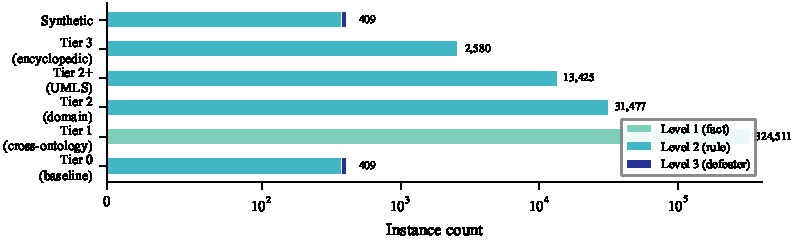
\includegraphics[width=\textwidth]{figures/fig_composition.pdf}
\caption{Dataset composition by tier and instance level. Tier~1 (cross-ontology extraction from OpenCyc + ConceptNet) provides the majority of instances; Level~3 (defeater abduction) instances appear only in Tier~0 and the matched synthetic control. Symlog scale.}
\label{fig:composition}
\end{figure}

\paragraph{Volume and balance.}
Table~\ref{tab:kbsummary} and Figure~\ref{fig:composition} summarize extraction results across tiers. The Tier~0 evaluation set contains 374 Level~2 and 35 Level~3 instances across three domains (biology: 114, legal: 168, materials: 92). Tier~1 provides the primary scale (324K instances across five domains); Tier~2 adds 44,902 domain-specific instances; Tier~3 contributes 2,580 instances from the encyclopedic YAGO~4.5.

\paragraph{Level~3 defeater sources.}
The richest automated sources are Wikidata P2303 constraint--exception pairs (11,557 defeaters), Gene Ontology \texttt{NOT}-qualified annotations (1,250), and SUMO axioms (792). The Tier~0 Level~3 set (35 instances) includes both automatically extracted and expert-authored defeaters.

\paragraph{Structural difficulty.}
For Tier~0 Level~2 ($n = 374$): mean support size $|\Supp| = 147$ (std.\ 105), unique gold per instance ($|\Hgold| = 1$), $|\Hcand| = 6$. Level~3 ($n = 35$): mean novelty $\Nov^* = 0.14$ (range 0--0.5). Gold set multiplicity and candidate pool size are uncorrelated ($r = 0.000$).

\paragraph{Decoder validation.}
Modalities M2--M4 achieve 100\% round-trip recovery across all 409 gold hypotheses. M1 (narrative) operates approximately by design.


%% ====================================================================
\section{Baseline Evaluation}\label{sec:evaluation}
%% ====================================================================


%% --------------------------------------------------------------------
\subsection{Experimental Setup}\label{subsec:setup}
%% --------------------------------------------------------------------

\paragraph{Models.}
We evaluate four frontier models: GPT-5.2-chat~\cite{openai2025gpt52} and Kimi-K2.5~\cite{moonshot2025kimi} (reasoning-optimized, closed-source), Claude~Sonnet~4.6~\cite{anthropic2024claude} (instruction-optimized, closed-source), and DeepSeek-R1-Distill-Llama-70B~\cite{deepseek2025r1} (reasoning-optimized, open-source). All models are evaluated with greedy decoding (temperature~$= 0$).

\paragraph{Compute.}
Closed-source models are accessed via Azure AI Foundry. Open-source models are served via vLLM~\cite{kwon2023vllm} on CURC Alpine (NVIDIA A100 80\,GB GPUs).

\paragraph{Conditions.}
Each instance is presented under all four text rendering modalities (M1--M4) and two prompting strategies (direct and chain-of-thought). The CoT scaffold mirrors defeasible derivation structure: identify applicable rules, determine missing/blocking elements, check for attackers and superiority, and propose a conservative hypothesis. M5 visual grounding (Section~\ref{subsec:m5}) is evaluated separately on vision-capable models (GPT-5.2, Claude~Sonnet~4.6, Qwen2.5-VL-72B, Qwen2.5-VL-7B) using instances with image coverage $c \geq 0.5$.


%% --------------------------------------------------------------------
\subsection{Primary Results}\label{subsec:results}
%% --------------------------------------------------------------------

Table~\ref{tab:main} summarizes accuracy by level and prompting strategy. All pairwise differences at Level~3 are statistically significant by McNemar's test ($p < 0.001$) except Claude vs.\ Kimi ($p = 0.556$).

\begin{table}[t]
\centering
\caption{Accuracy (\%) by model and task level across all four rendering modalities and both prompting strategies. Level~2 = rule abduction (374 instances); Level~3 = defeater abduction (35 instances). Wilson 95\% CI half-widths: $\pm 4$ pp at Level~2; $\pm 15$--$17$ pp at Level~3.}
\label{tab:main}
\begin{tabular}{lcccccc}
\toprule
Model & L2 & L2 Direct & L3 & L3 Direct & L3 CoT & Rend.-Robust \\
\midrule
DeepSeek-R1         & 73.0\% & 73.7\% & \textbf{65.0\%} & 37.1\% & \textbf{92.9\%} & \textbf{23.5\%} \\
GPT-5.2-chat        & 62.8\% & \textbf{78.5\%} & 47.5\% & \phantom{0}7.9\% & 87.1\% & \phantom{0}9.1\% \\
Claude~Sonnet~4.6   & \textbf{77.2\%} & 79.3\% & 16.4\% & \textbf{23.6\%} & \phantom{0}9.3\% & 15.5\% \\
Kimi-K2.5           & 65.5\% & 71.9\% & 14.2\% & \phantom{0}0.8\% & 27.6\% & \phantom{0}7.8\% \\
\bottomrule
\end{tabular}
\end{table}

\begin{figure}[t]
\centering
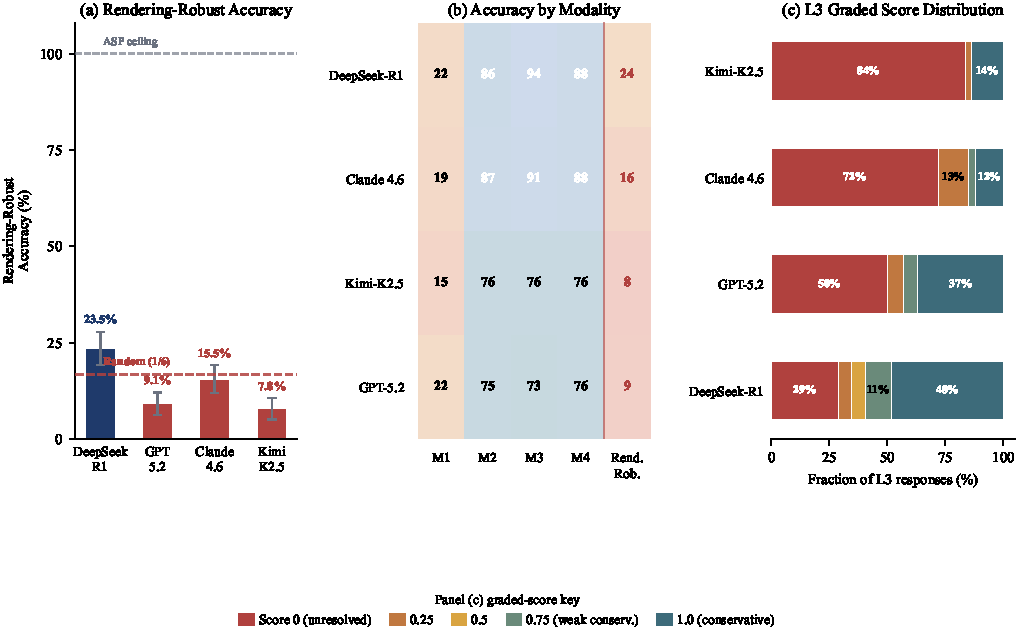
\includegraphics[width=\textwidth]{figures/fig_results.pdf}
\caption{(a)~Level~3 (defeater abduction) accuracy by prompting strategy. Reasoning-optimized models (DeepSeek-R1, GPT-5.2) gain +56 to +79~pp under chain-of-thought prompting; the instruction-optimized Claude regresses by $-14$~pp. (b)~Accuracy by rendering modality (all levels pooled). All models collapse to 14--22\% on narrative rendering (M1) versus 73--94\% on formal modalities (M2--M4), the largest effect in the evaluation.}
\label{fig:results}
\end{figure}


%% --------------------------------------------------------------------
\subsection{Key Findings}\label{subsec:findings}
%% --------------------------------------------------------------------

\paragraph{Grounding is largely solved.}
Under direct prompting across formal modalities (M2--M4), all four models achieve strong Level~2 accuracy: Claude 79.3\%, GPT-5.2 78.5\%, DeepSeek-R1 73.7\%, Kimi 71.9\%. Domain breakdown reveals a consistent ordering: legal is hardest (57--72\%), biology easiest (68--82\%), reflecting denser rule structures in LKIF Core rather than idiosyncratic knowledge gaps.

\paragraph{Belief revision is latent, not absent.}
Level~3 performance depends critically on both architecture and prompting (Figure~\ref{fig:results}a). Reasoning-optimized models gain +56 to +79~pp under CoT, while Claude \emph{regresses} by $-14$~pp. This architectural dissociation reveals that belief revision capability is not absent but is highly sensitive to the prompting paradigm.

\paragraph{Narrative rendering is a universal bottleneck.}
All models drop to 14--22\% on narrative rendering (M1) versus 73--94\% on formal modalities (M2--M4), as shown in Figure~\ref{fig:results}b. This 55--70 pp gap is the largest effect in the evaluation, larger than any inter-model or inter-level difference. Rendering-robust accuracy is dominated by M1 performance.

\paragraph{CoT hurts candidate selection.}
The CoT lift at Level~2 is \emph{negative} for all models ($-1.5$ to $-31$ pp): for structured selection tasks where surface alignment between output and candidate strings suffices, chain-of-thought elaboration disrupts that alignment. This replicates the ``overthinking'' effect~\cite{chen2024overthinking}.

\paragraph{Contamination analysis status.}
The synthetic contamination control methodology is established: 409 structurally matched synthetic instances have been generated with invented predicate names (Section~\ref{subsec:synthetic}). Evaluation of frontier models on synthetic instances and computation of the contamination gap $\Delta_{\mathrm{synth}}$ is in progress. Preliminary methodology validation confirms that synthetic theories preserve structural difficulty distributions of their naturalistic counterparts while using entirely novel vocabulary.


%% ====================================================================
\section{Discussion}\label{sec:discussion}
%% ====================================================================

\paragraph{Grounding and revision remain dissociable.}
The Level~2-to-Level~3 gap persists even for the best model under the best prompting strategy: DeepSeek-R1 achieves 73.7\% direct L2 versus 37.1\% direct L3, a 37 pp gap. Claude, whose direct L2 (79.3\%) and direct L3 (23.6\%) differ by 56 pp, shows that high grounding accuracy does not imply belief revision capability.

\paragraph{Prompt structure is a confounding variable.}
The large CoT lift for reasoning models ($+56$ to $+79$ pp) demonstrates that prompting template choice can shift measured Level~3 accuracy by more than the difference between any two models. Benchmarks for formal abductive reasoning should report performance separately by prompting strategy.

\paragraph{Visual grounding.}
The M5 modality (Section~\ref{subsec:m5}) tests whether defeasible reasoning transfers to multimodal settings where VLMs fail on atypical instances~\cite{park2025visage}---precisely the entities governed by defeater rules.

\paragraph{Future directions.}
The verifier-backed gold standards make DeFAb suitable as an exact reward function for DPO and RLHF without reward model approximation error. Adversarial multi-agent evaluation via tree search over ablated proof trees offers a complementary adaptive evaluation paradigm.

\paragraph{Limitations.}
The Tier~0 evaluation uses 409 instances (35 Level~3); Wilson CI half-widths are $\pm 15$--$17$ pp at Level~3. Automated Level~3 generation is limited by sparse exception edges in source KBs. The synthetic contamination control mitigates but does not eliminate the confound: structural patterns of defeasible theories may themselves be memorized.


%% ====================================================================
\section{Conclusion}\label{sec:conclusion}
%% ====================================================================

We have introduced \textsc{DeFAb}, a benchmark for evaluating foundation models on defeasible abduction. The dataset comprises 372,402 instances from 33.7 million materialized rules across 15 knowledge sources, with polynomial-time verifiable gold-standard hypotheses at three difficulty levels. Evaluation of four frontier models reveals that grounding is largely solved (73--79\% at Level~2) while belief revision is latent and prompt-sensitive, with an architectural dissociation between reasoning-optimized and instruction-optimized models. Two methodological findings extend beyond this benchmark: the prompt-format confound, where uniform CoT templates misestimate capability across task types; and the narrative-modality bottleneck, where rendering robustness constitutes a distinct evaluation dimension. DeFAb provides formal infrastructure to track progress on belief revision as training paradigms evolve.


%% ====================================================================
\section{Dataset Access}\label{sec:access}
%% ====================================================================

The DeFAb dataset, generation pipeline, and evaluation harness are released under the MIT license on HuggingFace Datasets (\url{https://huggingface.co/datasets/PatrickAllenCooper/DeFAb}) with Croissant metadata (core and RAI fields). Each instance is a JSON object containing the challenge theory, target literal, candidate and gold hypothesis sets, difficulty metrics, and renderings in all modalities. Source KB licenses are enumerated in the Datasheet (Appendix~\ref{app:datasheet}). The dataset will be maintained for at least 5 years; Tier~0 instances are frozen for cross-study comparability.


\bibliographystyle{plainnat}
\bibliography{references}


%%%%%%%%%%%%%%%%%%%%%%%%%%%%%%%%%%%%%%%%%%%%%%%%%%%%%%%%%%%%


%% =================================================================
%%  APPENDICES
%% =================================================================

\appendix


%% =================================================================
\section{Formal Definitions}\label{app:definitions}
%% =================================================================

\subsection{Defeasible Theories}

\begin{definition}[Defeasible Theory]\label{def:deftheory}
A defeasible theory is a quintuple $\D = (F, \Rs, \Rd, \Rdf, {\succ})$ where:
\begin{enumerate}[label=(\roman*)]
    \item $F \subseteq \HB$ is a finite set of facts;
    \item $\Rs$ is a finite set of strict rules: $r_s\colon b_1, \ldots, b_n \strictto h$;
    \item $\Rd$ is a finite set of defeasible rules: $r_d\colon b_1, \ldots, b_n \defto h$;
    \item $\Rdf$ is a finite set of defeaters: $r_{df}\colon b_1, \ldots, b_n \defeatto \neg h$; and
    \item ${\succ} \;\subseteq (\Rd \cup \Rdf) \times (\Rd \cup \Rdf)$ is an acyclic superiority relation.
\end{enumerate}
\end{definition}

\begin{definition}[Defeasible Derivation]\label{def:defderiv}
$+\partial q$ (defeasible provability) holds iff: (1) $+\Delta q$; or (2) all of:
\begin{enumerate}[label=(\alph*)]
    \item $-\Delta \comp{q}$;
    \item $\exists\, r \in \Rd$ with $C(r) = q$ and $\forall\, a \in A(r)$: $+\partial a$; and
    \item $\forall\, s \in \Rd \cup \Rdf$ with $C(s) = \comp{q}$: either $\exists\, a \in A(s)$: $-\partial a$; or $\exists\, t \in \Rd$ with $C(t) = q$, $\forall\, a \in A(t)$: $+\partial a$, and $t \succ s$.
\end{enumerate}
\end{definition}

\subsection{Conservativity and Anomalies}

\begin{definition}[Expectation Set]\label{def:expectation}
$\Exp(\D) = \{q \mid \D \pPartial q\}$.
\end{definition}

\begin{definition}[Anomaly]\label{def:anomclass}
A ground literal $\alpha$ is a defeasible anomaly if $\D \pPartial \comp{\alpha}$ and $\D \not\pDelta \comp{\alpha}$.
\end{definition}

\begin{definition}[Conservativity]\label{def:conserv}
A resolution $(r, \Gamma)$ of anomaly $\alpha$ with respect to $\D$ is conservative if:
\[
    \Exp(\D \cup \{r\} \cup \Gamma \cup \{\alpha\}) \supseteq \Exp(\D) \setminus \{\comp{\alpha}\}.
\]
\end{definition}

\begin{definition}[Revision Distance]\label{def:revdist}
$d_{\mathrm{rev}}(\D, \D') = |\D' \setminus \D| + |\Exp(\D) \setminus \Exp(\D')|$.
\end{definition}

\begin{definition}[Predicate Novelty]\label{def:novelty}
$\Nov(r, \Dm) = |\pred(r) \setminus \pred(\Dm)| / |\pred(r)|$.
\end{definition}

\subsection{Instance Generation}

\begin{definition}[Full-Theory Criticality]\label{def:fullcrit}
$\CritStar(\D, q) = \{e \in F \cup \Rs \cup \Rd \mid \D \setminus \{e\} \not\pPartial q\}$.
\end{definition}

\begin{definition}[Level 3 Instance Generation]\label{def:level3gen}
Given complete theory $\Dfull$ with $\Rdf \neq \emptyset$: (1) select $r^*$; (2) find $\alpha$ with $\Dfull \pPartial \alpha$ and $\Dfull \setminus \{r^*\} \pPartial \comp{\alpha}$; (3) form $\Dm$; (4) verify $\Dm \pPartial \comp{\alpha}$ and $\Dm \not\pDelta \comp{\alpha}$; (5) compute $\Rgold$.
\end{definition}

\begin{definition}[Structural Difficulty]\label{def:structdiff}
$\sigma(I) = (\ell,\; |\Supp(\D, q)|,\; |\Hgold|,\; \min_{h \in \Hgold} |h|,\; \Nov^*(I))$.
\end{definition}


%% =================================================================
\section{Proofs}\label{app:proofs}
%% =================================================================

\begin{proposition}[Conservativity of Strict Conversion]\label{prop:strict}
If $\partfunc \equiv s$, then $q \in \mathcal{M}_\Pi \iff \D_\partfunc \pDelta q$.
\end{proposition}

\begin{proof}
When $\partfunc \equiv s$, $\Rd^{\partfunc} = \emptyset$, and the strict fragment is isomorphic to $\Pi$. The definite provability relation on the strict fragment coincides with $\mathrm{lfp}(T_\Pi) = \mathcal{M}_\Pi$.
\end{proof}

\begin{theorem}[Defeasible Derivation in P]\label{thm:derivP}
For propositional defeasible theories, deciding $\D \pPartial q$ is in P, computable in $O(|R| \cdot |F|)$ time~\cite{maher2001propositional}.
\end{theorem}

\begin{theorem}\label{thm:critP}
$\CritStar(\D, q)$ is computable in $O(|\D|^2 \cdot |F|)$ time.
\end{theorem}

\begin{corollary}\label{cor:cubic}
The full instance generation pipeline runs in $O(|\D|^3)$.
\end{corollary}

\begin{theorem}[First-Order Complexity]\label{thm:firstorder}
For the function-free (datalog) fragment, the pipeline remains in P with respect to grounded size.
\end{theorem}

\begin{proposition}[Monotonicity of Expected Yield]\label{prop:yieldmono}
$\mathbb{E}[Y(\partfunc_{\mathrm{rand}}(\delta), Q)]$ is non-decreasing in $\delta$.
\end{proposition}

Full proofs for all results are provided in the companion technical report~\cite{cooper2026defab}. Proof sketches for the key tractability results appear above.


%% =================================================================
\section{Worked Example}\label{app:example}
%% =================================================================

\begin{example}[IDP Discovery as Defeater Abduction]\label{ex:idp}
Consider a simplified biochemistry program $\Pi_{\mathrm{bio}}$:
\begin{align*}
    &\text{protein}(\text{p53\_idr}) \leftarrow &\quad &\text{functional}(\text{p53\_idr}) \leftarrow \\
    &\text{disordered}(\text{p53\_idr}) \leftarrow &\quad &\text{has\_stable\_3d}(X) \leftarrow \text{protein}(X) \\
    &\text{func\_mech}(X, \text{lock\_key}) \leftarrow \text{protein}(X), \text{has\_stable\_3d}(X)
\end{align*}

Under $\partfunc_{\mathrm{rule}}$, we obtain $\D_{\mathrm{bio}}$ with defeasible rules $r_1\colon \text{protein}(X) \defto \text{has\_stable\_3d}(X)$ and $r_2\colon \text{protein}(X), \text{has\_stable\_3d}(X) \defto \text{func\_mech}(X, \text{lock\_key})$.

Extending to $\Dfull_{\mathrm{bio}}$ with the IDP exception: $r_3\colon \text{disordered}(X) \defto \neg\text{has\_stable\_3d}(X)$ and $r_4\colon \text{disordered}(X), \text{protein}(X) \defto \text{func\_mech}(X, \text{conf\_ensemble})$, with $r_3 \succ r_1$ and $r_4 \succ r_2$.

Remove $r_4$ and its superiority to form $\Dm_{\mathrm{bio}}$. The observation $\alpha = \text{func\_mech}(\text{p53\_idr}, \text{conf\_ensemble})$ is now anomalous. The model must construct a defeater that explains how p53\_idr can be functional despite lacking stable structure, producing $r_4$ (a strong conservative resolution with $\Nov = 1/4 > 0$).
\end{example}


%% =================================================================
\section{M5 Implementation Details}\label{app:m5details}
%% =================================================================

\paragraph{Image sourcing.} Images are harvested from three linked knowledge bases:
\begin{itemize}[nosep]
\item \textbf{Wikidata P18}: the ``image'' property links entities to Wikimedia Commons photographs, queryable via SPARQL against entity Q-IDs stored in rule metadata. Thumbnails at configurable resolution (default 640px).
\item \textbf{VisualSem}~\cite{geigle2024babelimagenet}: approximately 938,000 images across 90,000 nodes bridging WordNet synsets and BabelNet, providing direct mappings for entities in the Tier~0 and Tier~1 theories.
\item \textbf{BabelNet 5.3}: 61.4 million images across 23 million synsets, accessible via REST API.
\end{itemize}
An \texttt{ImageManifest} indexes entity-to-image associations with source-priority selection (Wikidata $>$ VisualSem $>$ BabelNet). The coverage ratio $c(\D, \mathcal{I}) = |\{e \in \mathrm{entities}(\D) : \mathcal{I}(e) \neq \emptyset\}| / |\mathrm{entities}(\D)|$ measures the fraction of theory entities with available images; M5 instances require $c \geq \theta$ for a configurable threshold~$\theta$.

\paragraph{VLM evaluation panel.} The closed-source tier comprises GPT-5.2-chat~\cite{openai2025gpt52} and Claude~Sonnet~4.6~\cite{anthropic2024claude}, both accessed via Azure AI Foundry with multimodal content blocks. The open-source tier comprises Qwen2.5-VL-72B-Instruct-AWQ (2$\times$A100 80\,GB, tensor parallel 2) and Qwen2.5-VL-7B-Instruct (1$\times$A100 80\,GB, within-family scaling comparator), served via vLLM on CURC Alpine with OpenAI-compatible multimodal API.

\paragraph{Loading example.}
\begin{verbatim}
import json
with open("instances/tier0/level3_instances.json") as f:
    data = json.load(f)
for inst in data["instances"]:
    theory = inst["theory"]
    target = inst["target"]
    candidates = inst["candidates"]
\end{verbatim}


%% =================================================================
\section{Complexity Table}\label{app:complexity}
%% =================================================================

\begin{table}[h]
\centering
\small
\caption{Complexity of key pipeline operations. All are polynomial in the theory size $|\D|$.}
\label{tab:complexity}
\begin{tabular}{@{}lc@{}}
\toprule
Operation & Complexity \\
\midrule
Defeasible derivation $\D \pPartial q$ & $O(|R| \cdot |F|)$ \\
Gold-standard verification & P \\
Full-theory criticality $\CritStar(\D, q)$ & $O(|\D|^2 \cdot |F|)$ \\
Full pipeline per instance & $O(|\D|^3)$ \\
\bottomrule
\end{tabular}
\end{table}


%% =================================================================
\section{Datasheet for DeFAb}\label{app:datasheet}
%% =================================================================

\subsection*{Motivation}

\begin{itemize}[nosep]
\item \textbf{Purpose:} DeFAb was created to evaluate foundation models on defeasible abduction --- the ability to construct hypotheses that explain anomalies by overriding default conclusions while preserving unrelated expectations. No existing benchmark combines formally verifiable gold-standard hypotheses with conservativity constraints and contamination-resistant evaluation.
\item \textbf{Creators:} Patrick Cooper, University of Colorado Boulder.
\item \textbf{Funding:} University of Colorado Boulder Department of Computer Science.
\end{itemize}

\subsection*{Composition}

\begin{itemize}[nosep]
\item \textbf{Instance types:} Each instance is an abductive reasoning task consisting of an ablated defeasible theory $\Dm$, a target literal $q$, a candidate hypothesis set $\Hcand$, and gold-standard answers $\Hgold$. Level~1 instances require fact completion; Level~2 require rule abduction; Level~3 require conservative defeater construction.
\item \textbf{Instance count:} Tier~0: 409 (374 L2, 35 L3). Tier~1: 324,511 (182K L1, 142K L2) across five domains. Tier~2: 44,902 from FrameNet, UMLS, SUMO, Gene Ontology, Wikidata, and BabelNet. Tier~3: 2,580 from YAGO 4.5 full. Synthetic: 409 contamination-control instances matched to Tier~0. Total: 372,402.
\item \textbf{Rule base:} 33.7 million materialized rules from 15 knowledge sources (Tiers 0--3, including 29.5 million from UMLS 2025AB).
\item \textbf{Sensitive content:} None. All instances are derived from formal logic programs over scientific and commonsense knowledge.
\item \textbf{Personal data:} None. No human subjects, no crowdsourcing, no personal information.
\end{itemize}

\subsection*{Collection Process}

\begin{itemize}[nosep]
\item \textbf{Acquisition:} Instances are generated by a deterministic polynomial-time pipeline (Section~\ref{sec:design}) from publicly available knowledge bases. No crowdsourcing or human annotation is involved except for a small set (35) of high-novelty Level~3 defeaters authored by the paper's author.
\item \textbf{Time frame:} Source knowledge bases span 1984 (Cyc) to 2025 (UMLS 2025AB, YAGO 4.5).
\item \textbf{Ethical review:} No IRB review required (no human subjects). All source KBs are publicly available under open licenses.
\end{itemize}

\subsection*{Preprocessing}

\begin{itemize}[nosep]
\item \textbf{Preprocessing:} Source knowledge bases are converted to definite logic programs, then to defeasible theories via the parameterized partition function $\kappa$. Cross-ontology extraction normalizes concept names across sources using lowercased, underscore-separated identifiers. Non-English content is filtered at the extraction stage.
\item \textbf{Raw data:} All source knowledge bases are publicly available under open licenses (see Section~\ref{sec:access}).
\end{itemize}

\subsection*{Uses}

\begin{itemize}[nosep]
\item \textbf{Intended uses:} Evaluating foundation models on non-monotonic reasoning, belief revision, and grounded hypothesis generation. The polynomial-time verifier-backed scoring function makes the dataset suitable as a training signal for preference optimization (DPO, RLHF) without reward model approximation.
\item \textbf{Not intended for:} Making real-world scientific, legal, or medical decisions. The defeasible rules encode general defaults and exceptions from knowledge bases, not clinical or legal guidance.
\end{itemize}

\subsection*{Distribution}

\begin{itemize}[nosep]
\item \textbf{License:} MIT (generation pipeline and produced instances). Source KB licenses: YAGO (CC-BY 4.0), WordNet (Princeton License), LKIF Core (Apache 2.0), MatOnto (CC-BY 4.0), Wikidata (CC0 1.0), ConceptNet (CC-BY-SA 4.0), Gene Ontology (CC-BY 4.0), UMLS (NLM License, free for research), SUMO (GPLv2), FrameNet (CC-BY 3.0).
\item \textbf{Distribution platform:} HuggingFace Datasets. The dataset, generation pipeline, and evaluation harness are hosted as a single repository.
\end{itemize}

\subsection*{Maintenance}

\begin{itemize}[nosep]
\item \textbf{Maintainer:} Patrick Cooper, University of Colorado Boulder (\texttt{patrick.cooper@colorado.edu}).
\item \textbf{Duration:} The dataset will be maintained for at least 5 years from publication. The generation pipeline enables re-generation from updated source KBs.
\item \textbf{Updates:} New source KBs and instance tiers will be added via versioned releases (v1.0, v1.1, etc.). Release notes will accompany each version.
\item \textbf{Issues:} Bug reports and error corrections are tracked via the GitHub repository (\url{https://github.com/PatrickAllenCooper/blanc}).
\item \textbf{Versioning:} Semantic versioning. The Tier~0 evaluation instances are frozen at v1.0 for cross-study comparability; additional tiers are additive.
\end{itemize}


\newpage
\section*{NeurIPS Paper Checklist}

\begin{enumerate}

\item {\bf Claims}
    \item[] Answer: \answerYes{}
    \item[] Justification: The introduction lists five numbered contributions, each developed in corresponding sections (Sections~\ref{sec:design}--\ref{sec:evaluation} and~\ref{subsec:m5}). All accuracy figures include Wilson 95\% CIs. Claims about dataset scale are backed by Table~\ref{tab:kbsummary}.

\item {\bf Limitations}
    \item[] Answer: \answerYes{}
    \item[] Justification: Section~\ref{sec:discussion} discusses limitations: Tier~0 sample size (35 L3 instances), M1 decoder approximation, sparse automated Level~3 generation from ConceptNet, and structural contamination residual.

\item {\bf Theory assumptions and proofs}
    \item[] Answer: \answerYes{}
    \item[] Justification: All propositions and theorems are numbered. Proof sketches for key results appear in Appendix~\ref{app:proofs}; full proofs are provided in the companion technical report. Assumptions are stated explicitly (e.g., Proposition~\ref{prop:strict} assumes all-strict partition).

\item {\bf Experimental result reproducibility}
    \item[] Answer: \answerYes{}
    \item[] Justification: Section~\ref{sec:evaluation} specifies all models, decoding parameters, prompting strategies, and instance generation parameters. The full pipeline and all instances are released.

\item {\bf Open access to data and code}
    \item[] Answer: \answerYes{}
    \item[] Justification: The DeFAb dataset, generation pipeline, and evaluation harness are released under the MIT license (Section~\ref{sec:access}). Evaluated models are accessible via commercial APIs and open-source hosting.

\item {\bf Experimental setting/details}
    \item[] Answer: \answerYes{}
    \item[] Justification: Section~\ref{subsec:setup} specifies all models, API endpoints, and decoding parameters (greedy, temperature~$= 0$). Section~\ref{sec:design} specifies distractor count ($k = 5$), partition strategies, and the three-stage decoder pipeline.

\item {\bf Experiment statistical significance}
    \item[] Answer: \answerYes{}
    \item[] Justification: Table~\ref{tab:main} and Figure~\ref{fig:results} report Wilson 95\% confidence intervals. McNemar's test is used for pairwise model comparisons with reported $p$-values.

\item {\bf Experiments compute resources}
    \item[] Answer: \answerYes{}
    \item[] Justification: Section~\ref{subsec:setup} specifies Azure AI Foundry (eastus2, Global Standard) for closed-source models and CURC Alpine (NVIDIA A100 80\,GB) for open-source models.

\item {\bf Code of ethics}
    \item[] Answer: \answerYes{}
    \item[] Justification: All source knowledge bases are publicly available under open licenses. No personal data, crowdsourcing, or human subjects involved.

\item {\bf Broader impacts}
    \item[] Answer: \answerYes{}
    \item[] Justification: Positive: improved evaluation of reasoning deficits may accelerate development of more reliable AI. Negative: low risk; formal logic benchmark with no direct path to harmful deployment.

\item {\bf Safeguards}
    \item[] Answer: \answerNA{}
    \item[] Justification: Released artifacts are evaluation instances from public logic-based KBs and a deterministic pipeline. No pretrained models released; no sensitive content.

\item {\bf Licenses for existing assets}
    \item[] Answer: \answerYes{}
    \item[] Justification: All KBs cited with primary references. License information in Section~\ref{sec:access} and the Datasheet (Appendix~\ref{app:datasheet}). All licenses compatible with MIT release of derived instances.

\item {\bf New assets}
    \item[] Answer: \answerYes{}
    \item[] Justification: DeFAb dataset documented via Datasheet (Appendix~\ref{app:datasheet}), released with README, JSON format specification, and Croissant metadata (core and RAI fields).

\item {\bf Crowdsourcing and human subjects}
    \item[] Answer: \answerNA{}
    \item[] Justification: No crowdsourcing or human subjects involved. All instances generated by deterministic pipeline.

\item {\bf IRB approvals}
    \item[] Answer: \answerNA{}
    \item[] Justification: No human subjects involved. IRB review not required.

\item {\bf Declaration of LLM usage}
    \item[] Answer: \answerYes{}
    \item[] Justification: LLMs are the primary evaluated objects (Section~\ref{sec:evaluation}). The D3 semantic parser in the decoder pipeline employs a language model for hypothesis extraction from narrative responses.

\end{enumerate}


\end{document}
